\documentclass{article}

\usepackage{amsmath, tcolorbox, tikz}
\usepackage[version=4]{mhchem}
\usetikzlibrary{positioning}
\title {Cambridge GCSE Notes \\ 5070 Chemistry }
\author {Abrar Faiyaz Rahim, degrees pending}
\date {}

\begin{document}
\maketitle \newpage
\section*{Introduction}
What follows is my compilation of notes I used to get through my Ordinary Level GCSE 
exams, in the May-June session of 2025. I release all these notes to the public so as to 
help combat the tragic ``coaching culture" surrounding GCSE exams. This set of notes is 
written to be used in accordance to the coursebooks published by Cambridge, and is of
little use by itself.

My despiction of coaching culture arises from the fact that it ruins student life and
to a large extent the academic potential of students. A typical student has school in the 
day and in the evening they are made to sprint to and from coaching centres, often 
multiple teachers for the same subject all as a result of peer pressure and they come back home at 
9 or 10 at night. If they have been given homework, they must sacrifice their sleep to
complete these assignments. Students cannot, as a result, study by themselves -- ruining
their potential.

There exist accessible resources which are more than enough for a candidate to ace their 
exams, without any aid from the financially-minded coaching sharks. One of the services
provided by these teachers are ``compiled notes", exchanged for money, 
further inflating the price of education. So, in retaliation I release these 
notes as open-source and free to distribute.

Yet coachings are not entirely evil, students who struggle in certain subjects may ask 
for the aid of teachers of those subjects but it is meaningless to go to a different 
teacher for each and every subject.

These notes are condensed, written in sequence of the Cambridge specifications.

\section*{Suggestions for readers}
These notes are not at all stand-alone resources that will magically help you to get 
through your exams. I suggest purchasing and utilising the Cambridge coursebooks, and
read the chapters from there before referring to these notes, especially if the topic
in question is absolutely novel to you. 

YouTube has excellent resources, lectures galore
at your discretion, simply type in ``GCSE" alongside whatever topic you need to watch
the lectures on.

Lastly, for practice of questions, past papers both topically and yearly compiled are
available for purchase at bookstores and for free online (topicals can be found on
physicsandmathstutor.com).
\tableofcontents \newpage

\section{States of matter}
\subsection{Solids, liquids and gases}
\textbf{Matter} is anything that occupies space and has mass. There are three states matter can
be in: solid, liquid and gas. The latter two, liquid and gas are called \textbf{fluid} 
because they can flow and as a result they can be poured or pumped.
Matter is composed of particles.

\subsubsection*{Solids}
\textbf{Solids} have a fixed volume, with highest density of the three states, they have 
a definite fixed shape and are not fluid. The arrangement of particles in solids is regular,
every particle is very close to another and their movement is limited to vibrations about
fixed points. This is a result of the particles in solids having the least kinetic energy of
the three states.

\subsubsection*{Liquids}
\textbf{Liquids} have a fixed volume and their density is moderate to high, they lack any 
definite shape and take the shape of the container in which they are kept. They are fluid and
they flow easily. The particles are still close together, less than that in solids but are
in an irregular arrangement. The particles in liquids are able to move around and past each 
other as they have more kinetic energy than in solids.

\subsubsection*{Gases}
\textbf{Gases} have no fixed volume they expand to fill any container they are put into, they
have the loweest density and take the shape of the container they are put into. They too are
fluid. The particles in gases are very far apart, and have no arrangement. They move randomly
as a result of their high kinetic energy.

\subsubsection*{Changes of state}
The below shows the names of the changes of state from solid to liquid to gas.

\begin{figure}[h]
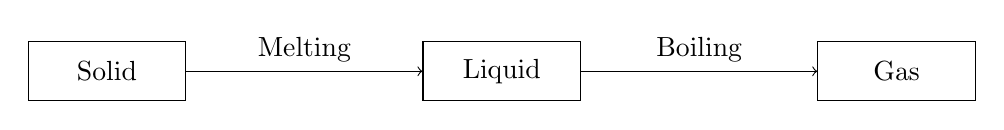
\begin{tikzpicture}[node distance=3cm]
	\centering
	\node[rectangle, text centered, draw=black, minimum height=0.75cm, minimum width=2cm] (solid) {Solid};
	\node[rectangle, text centered, draw=black, minimum height=0.75cm, minimum width=2cm] (liquid) [right=of solid]{Liquid};
	\node[rectangle, text centered, draw=black, minimum height=0.75cm, minimum width=2cm] (gas) [right=of liquid]{Gas};
	\draw [ -> ] (solid.east) -- (liquid.west)  node[midway, above]{Melting};
	\draw [ -> ] (liquid.east) -- (gas.west)  node[midway, above]{Boiling};
\end{tikzpicture}
\caption{Endothermic changes of state}
\end{figure}
These changes of state are endothermic because heat is applied to cause these changes.

The resulting state of these changes all have a higher kinetic energy than the previous
state. The resulting states have lower density and higher volumes. \newpage

\begin{figure}[h!]
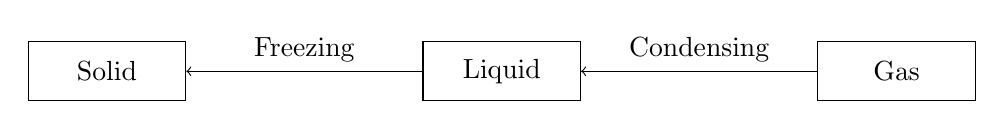
\begin{tikzpicture}[node distance=3cm]
	\centering
	\node[rectangle, text centered, draw=black, minimum height=0.75cm, minimum width=2cm] (solid) {Solid};
	\node[rectangle, text centered, draw=black, minimum height=0.75cm, minimum width=2cm] (liquid) [right=of solid]{Liquid};
	\node[rectangle, text centered, draw=black, minimum height=0.75cm, minimum width=2cm] (gas) [right=of liquid]{Gas};
	\draw [ <- ] (solid.east) -- (liquid.west)  node[midway, above]{Freezing};
	\draw [ <- ] (liquid.east) -- (gas.west)  node[midway, above]{Condensing};
\end{tikzpicture}
\caption{Exothermic changes of state}
\end{figure}
These changes of state are exothermic because because heat is absorbed (cold is applied)
to cause these changes.

The resulting state of these changes have a lower kinetic energy, higher density and
lower volume than the previous state.

\subsubsection*{Kinetic particle theory}
The kinetic particle theory states that all matter is composed of particles, which
have some kinetic energy and hence can move around. When energy is applied to these
particles, they move around more and vice versa.

\subsubsection*{Heating and cooling curves}
\begin{figure}[h!]
\begin{tikzpicture}[node distance=3cm]
	\centering
	\coordinate (O) (0, 0);
	\coordinate (ymax) (0, 5);
	\draw [ -> , thick] (O) -- (0, 5) node[anchor=south west]{temperature};
	\draw [ -> , thick] (O) -- (12, 0) node[anchor=north east]{time};

	\draw (0, 4.5) -- (1.75, 3.5) --
	(3.75, 3.5) -- (4.75, 2.5) -- (6.75, 2.5) -- (7.75, 1.5) -- (9.75, 1.5)
	-- (11, 0);

	\draw [dashed] (1.75, 3.5) -- (1.75, 0);
	\draw [dashed] (3.75, 3.5) -- (3.75, 0);
	\draw [dashed] (4.75, 2.5) -- (4.75, 0);
	\draw [dashed] (6.75, 2.5) -- (6.75, 0);
	\draw [dashed] (7.75, 1.5) -- (7.75, 0);
	\draw [dashed] (9.75, 1.5) -- (9.75, 0);

	\draw (0, 0) -- (1.75, 0) node[midway, below]{A};
	\draw (1.75, 0) -- (3.75, 0) node[midway, below]{B};
	\draw (3.75, 0) -- (4.75, 0) node[midway, below]{C};
	\draw (4.75, 0) -- (6.75, 0) node[midway, below]{D};
	\draw (6.75, 0) -- (7.75, 0) node[midway, below]{E};
	\draw (7.75, 0) -- (9.75, 0) node[midway, below]{F};
	\draw (9.75, 0) -- (11, 0) node[midway, below]{G};
\end{tikzpicture}
\caption{A typical cooling curve}
\end{figure}
Descriptions of what's happening in each region follows:
\begin{itemize}
	\item A: The temperature of the sample is decreasing, it is still gas.
	\item B: The temperature of the sample is constant, the sample is a mixture of
		gas and liquid. Here, the sample is condensing.
	\item C: The sample is completely liquid, temperature continues to decrease.
	\item D: The temperature is once again constant, as the
\end{itemize}

\section{Metals}
\subsection{Properties of metals}
Metals are those elements which lose electrons to form ions. They are to the left of
the zigzag line in the periodic table. They have the following general properties 
compared to non-metals:
\begin{itemize}
	\item Metals are good conductors of heat, and cold, i.e. they are good thermal
		conductors.
	\item Metals are good conductors of electricity because their structure consists
		of positive ions in a sea of delocalised electrons which can move around.
	\item Malleability and ductility: Metals are malleable, that means they can be 
		made into a variety of shapes. This is because metals have a layered molecular
		structure, layers which can slide over each other. They are ductile, meaning 
		they can be wrought out into wires.
	\item Melting points and boiling points: Metals have high melting and boiling points
		because of the strong metallic bonding between the positive ions and delocalised
		sea of electrons.
\end{itemize}
\subsubsection*{Reactions}
Metals react with dilute acids, water (in liquid and gaseous forms) and oxygen. They
fall into the following formats:
\begin{itemize}
	\item \ce{metal + dilute acid -> salt + hydrogen gas}
	\item \ce{metal + liquid water -> metal hydroxide + hydrogen gas}
	\item \ce{metal + steam -> metal oxide + hydrogen gas}
	\item \ce{metal + oxygen -> metal oxide}
\end{itemize}
These reactions are discussed at length in section 9.4.
\subsection{Uses of metals}
Metals are very useful as a result of their general properties. They are used in pots,
pans due to their ability to conduct heat very well. Aluminium is a metal which has the
following properties:
\begin{itemize}
	\item Low density
	\item Low reactivity (section 9.4)
	\item Corrosion resistance
\end{itemize}
It can thus be used in aircraft bodies, overhead electrical cables, and food containers.
Copper is used in electrical wiring.

\subsection{Alloys and their properties}
Alloys are mixtures of metals with other elements. Examples are brass (copper and zinc),
stainless steel (iron, chromium, nickel and carbon). These alloys can be harder because
the layers of particles can no longer slide over each other because of the differently
sized particles of the different elements. Stainless steel is used in cutlery because of
its corrosion rust resistance and hardness. Stainless steel has many such applications.

\subsection{Reactivity series}
Below is the reactivity series, in order of decreasing reactivity.

\begin{center}
\ce{K,Na,Ca,Mg,Al,C,Zn,Fe,H,Cu,Au,Ag}
\end{center}
A metal is said to be more reactive than another if it displaces the other from its 
aqueous compound. We can classify these further, highly reactive metals (HRMs): K, Na,
Ca, Mg, Al; moderately reactive metals (MRMs): Zn, Fe; and low reactive metals (LRMs):
Cu, Au, Ag.

Exceptions are as follow:
\begin{enumerate}
	\item Aluminium is a metal that is more reactive than most, but in reality it has
		a sample of aluminium tends to have a layer of \ce{Al2O3} around it (reacted
		with atmospheric oxygen). As a result aluminium is not particularly reactive
		unless the oxide layer is removed by any means.
	\item Carbon is a non-metal but its is more reactive than MRMs and LRMs, but this
		difference only applies for oxygen displacements. That is:
		
		\ce{2ZnO + C -> 2Zn + CO2} but 

		\ce{ZnSO4 + C -> ZnSO4 + C (no reaction)}
	\item Hydrogen is a gas. (bro just chilling)
\end{enumerate}

\subsubsection*{Reactions}
Metals react with water, in liquid and gaseous form; dilute acids and oxygen.
\begin{itemize}
	\item Cold water: Na, Ca and K react with cold (room temperature and pressure)
		water, to give a hydroxide and hydrogen gas:

		\ce{2Na (s) + 2H2O (l) -> NaOH (aq) + H2 (g)}

		\ce{2K (s) + 2H2O (l) -> KOH (aq) + H2 (g)}

		\ce{2Ca (s) + 2H2O (l) -> CaOH (aq) + H2 (g)}

		Observations of the above:
		\begin{itemize}
			\item Silvery solid dissolves.
			\item Bubbles of a colourless gas is seen.
			\item Heat is produced (solutions becomes heated).
		\end{itemize}
	\item Steam: All metals above H in the reactivity series react with steam, giving
		a metal oxide an hydrogen gas. For example:

		\ce{Ca (s) + H2O (g) -> CaO (s) + H2 (g)}

		Observations of the above:
		\begin{itemize}
			\item Silvery solid turns into white solid i.e. colour becomes dull.
		\end{itemize}
	\item Dilute acids: All metals above H react with dilute acids, giving a salt and
		hydrogen gas. For example:

		\ce{Mg (s) + 2HCl (aq) -> MgCl2 (aq) + H2 (g)}
\end{itemize}
All of the above reactions are displacement reactions, where H is replaced by metals
more reactive than it. Pb (lead) is a metal with a reactivity very close to H, as a 
result it sometimes displaces H and sometimes does not.

\end{document}
